\providecommand{\atd}{..}
\documentclass[../ATD.tex]{subfiles}
%%\usepackage{graphicx}

\begin{document}
    \chapter{Testing}\label{ch:testing}
    \section{Important note}\label{sec:important-note}
    An important issue has to be at least presented before to start to talk about the testing, since it compromises the correct use of the application.
    The issue will be discuss later, but it has a big impact on the structure of the document.
    \newline
    When the application run, after the user login an error message is show, and almost all the functionality of the application are not available.
    The error shows up on every device we used to run the application: web page, android phone, iOS phone, iOS simulator.
    We think that this issue cause the most of the fail on the test that will be presented in the next chapter.
    In the following are showed some picture of the error.

    %%
    \begin{figure}[H]
        \centering
        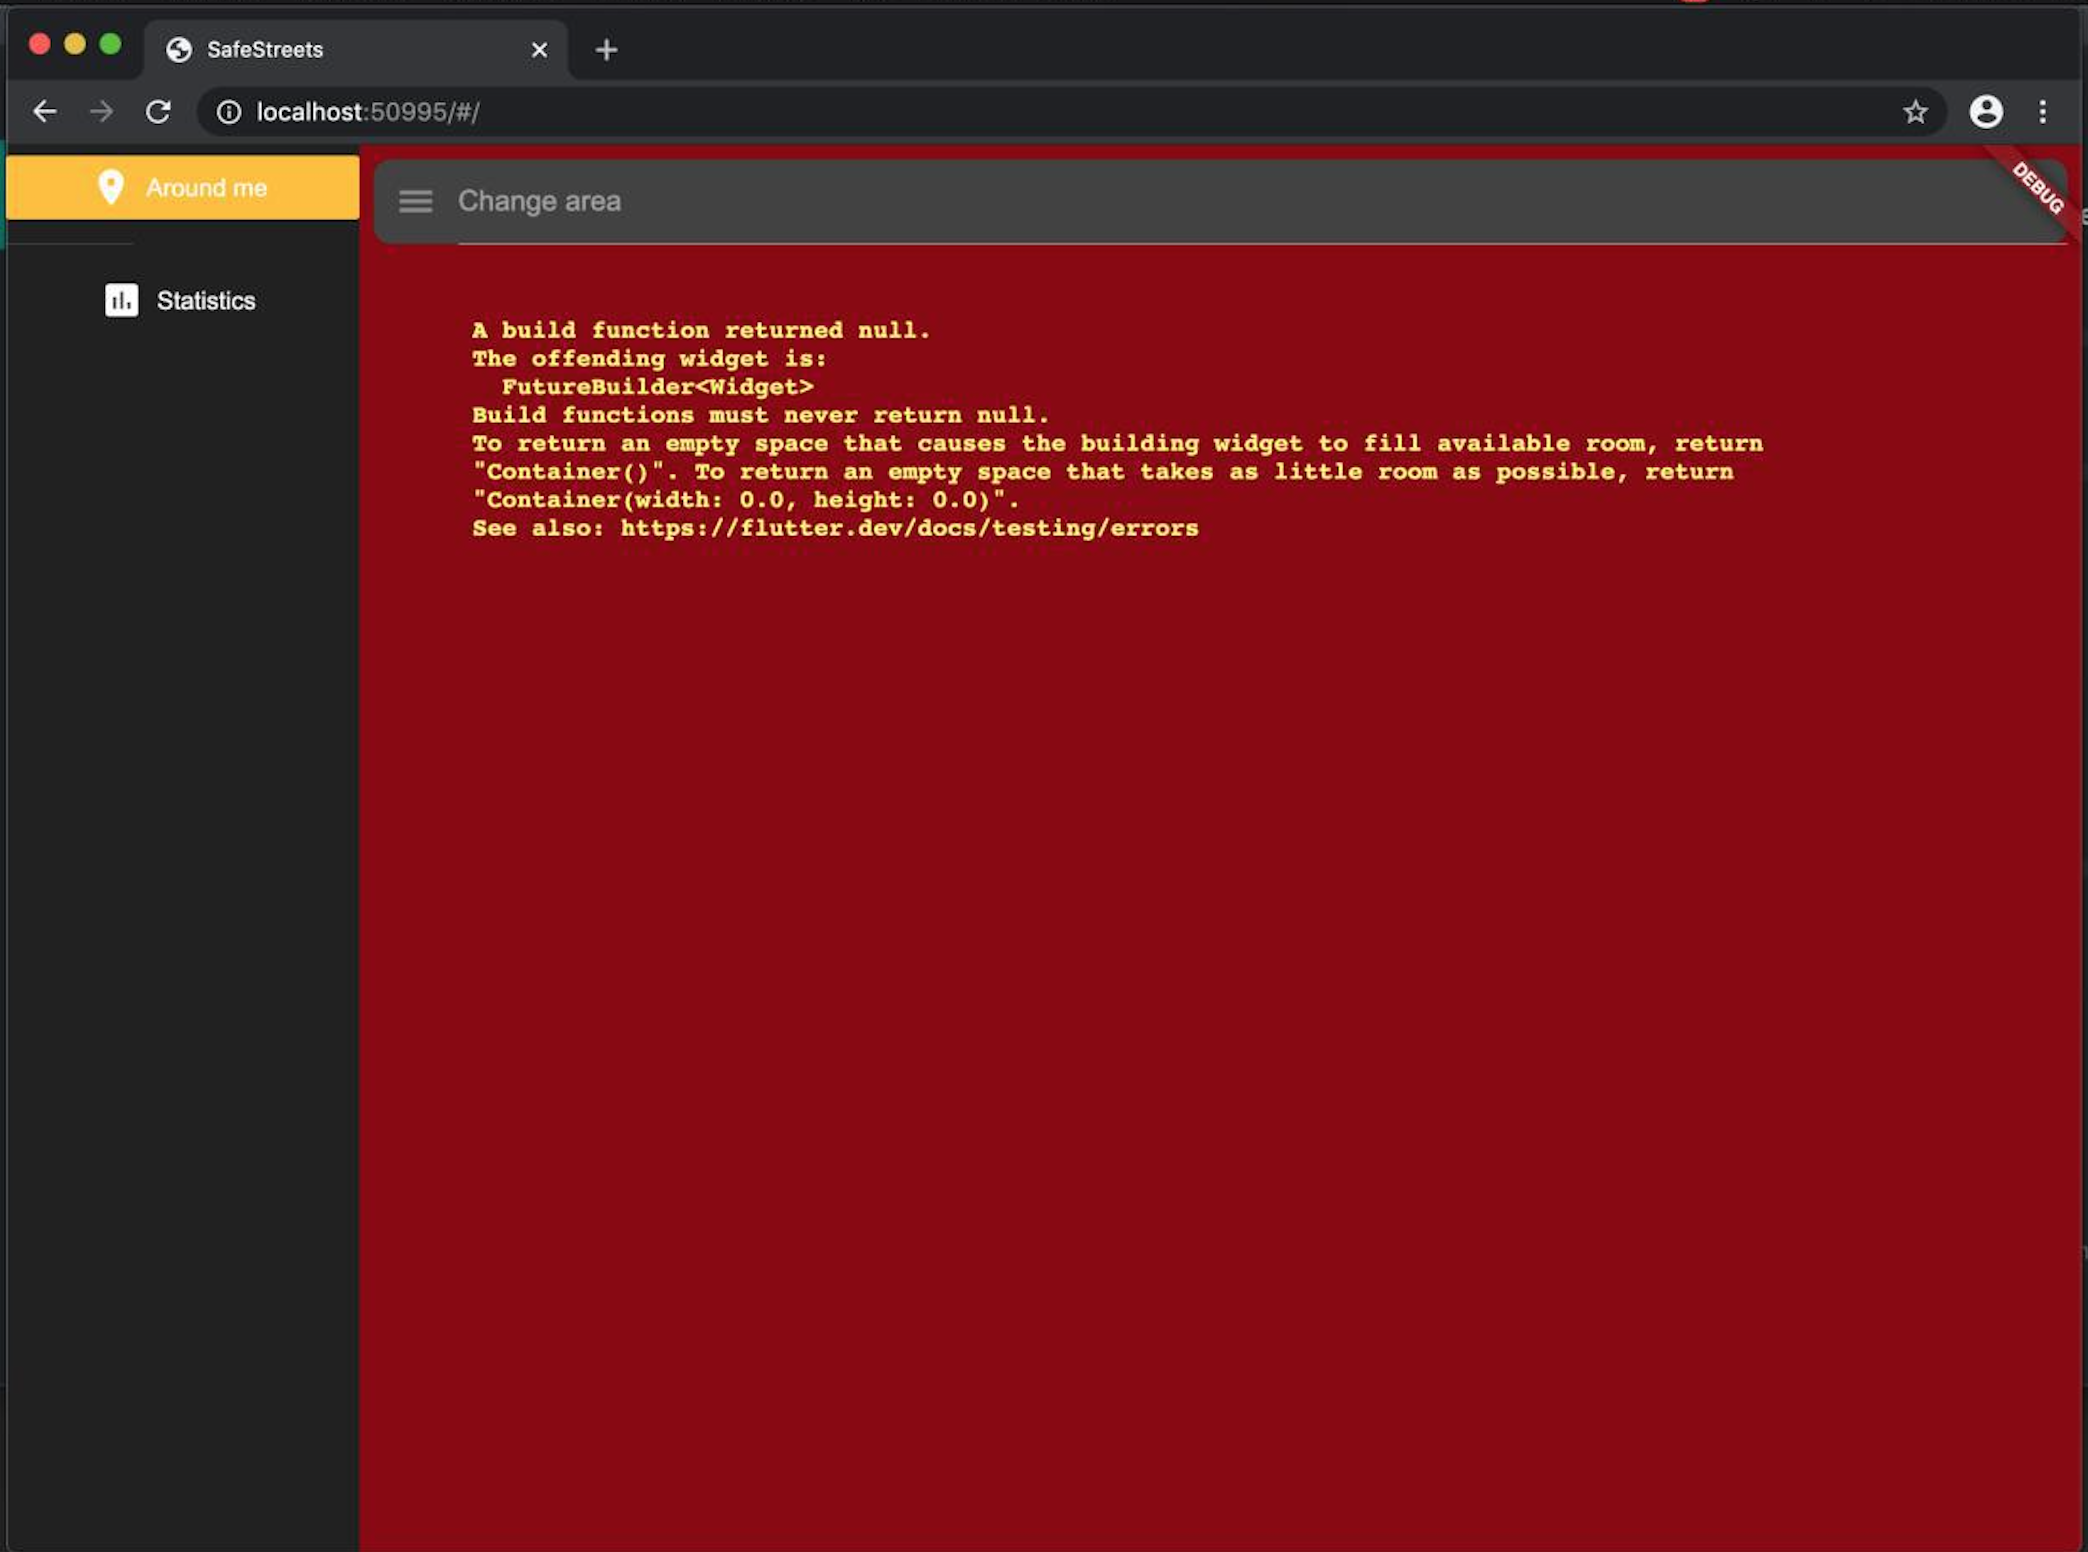
\includegraphics[scale = 0.4]{assets/web_page_error.png}\\
        \caption[Web page error, \textit{Error}]{Web page error}
    \end{figure}

    \begin{figure}[H]
        \centering
        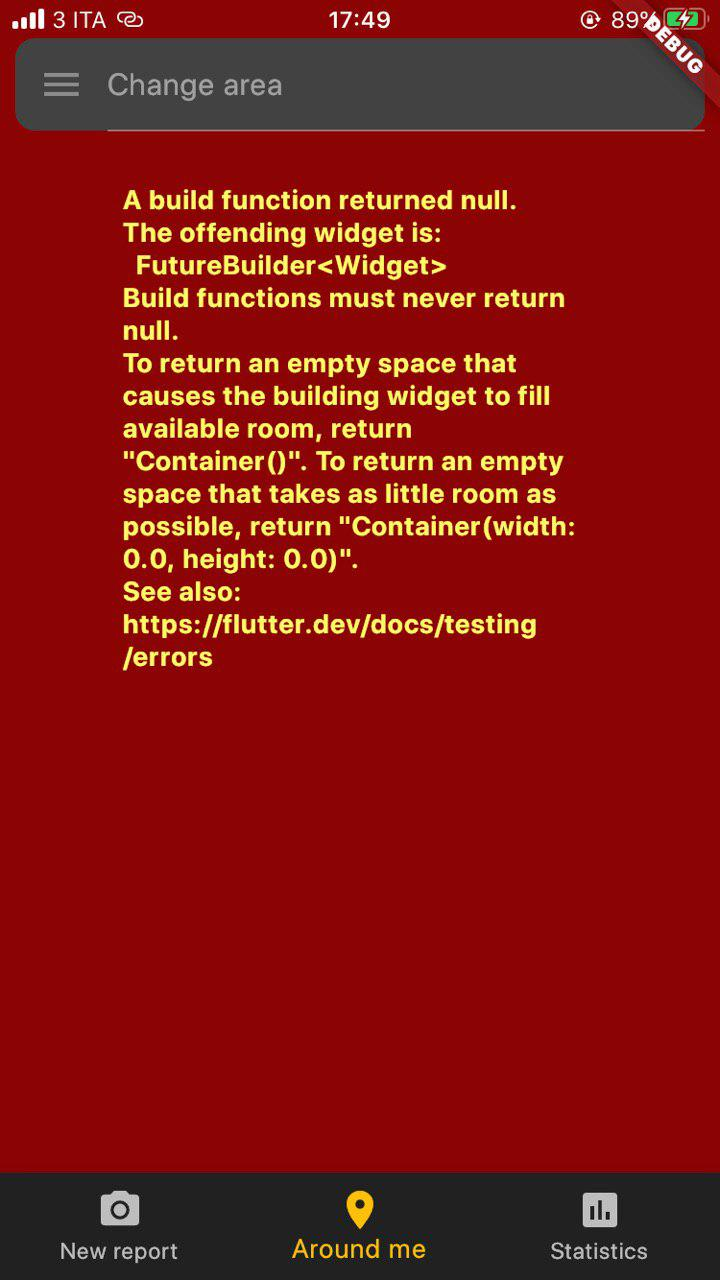
\includegraphics[scale = 0.4]{assets/smartphone_error.png}\\
        \caption[SMartphone error, \textit{Error}]{Smartphone error}
    \end{figure}
    \begin{figure}[H]
        \centering
        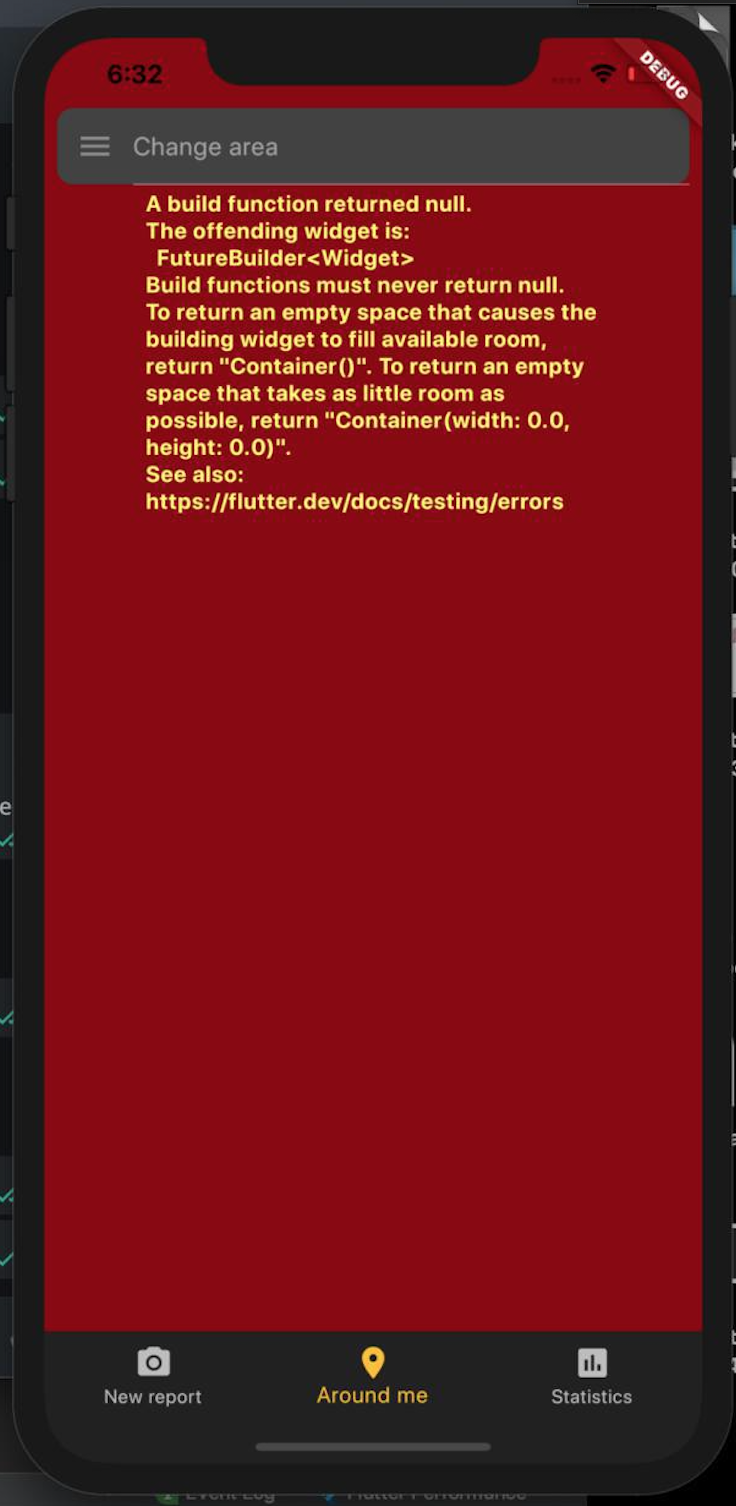
\includegraphics[scale = 0.7]{assets/iOS_simulator_error.png}
        \caption[IOs simulator error, \textit{Error}]{IOs simulator error}
    \end{figure}
%%
    \section{Testing Requirements Table}\label{sec:testing-requirements-table}
    Probably because of the already showed error, it will not be possible to test all the requirements since some of them will not be showed at all.
    Moreover, it will be difficult to follow the requirement order presented in the RASD and in the ITD while testing, so the following table purpose is to show which requirements will be tested.
    At the end of the chapter a section for the untested requirements will be provided anyway.

    %%todo ******** TABELLA *********

    \section{Test Cases}\label{sec:test-cases}
    The test cases will be presented as follow: they will be group by tested requirements, and for every test will be described the following information:
    \begin{enumerate}
        \item \textbf{Test purpose}
        \item \textbf{Device}: device on which the test run (android phone, iOS phone, simulator, web page, etc..)
        \item \textbf{Input}: input of the test
        \item \textbf{Outcome}: output of the test
        \item \textbf{Result}: passed or fail
        \item (Eventually) \textbf{Comment}: relevant comments about the test
    \end{enumerate}
    As previously explained, it will not be possible to test the requirements in the same order as they are presented in the RASD and ITD,
    but they will be marked with the same enumeration to make them easier to read.
    The requirements will be marked \textbf{[Rn]}, to refer to the n-th requirement.

    \subsection{User registration and login [R14]}\label{subsec:user-registration-and-login}
    R14: The system must allow the user to perform the registration and the login.

    \subsubsection{Correct login}\label{subsubsec:correct-login}
    \begin{itemize}
        \item \textbf{Test purpose}: An user that is already signed in must be able to login correctly.
        \item \textbf{Device}: iPhone
        \item \textbf{Input}: username: "jak4", password: "jak"
        \item \textbf{Outcome}:
        \item \textbf{Result}: passed
        \item \textbf{Comment}: The user "jak4" was already registered with the password "jak".
    \end{itemize}




\end{document}